\documentclass[conference]{IEEEtran}
\usepackage{pdfpages, etoolbox, soul}



% *** GRAPHICS RELATED PACKAGES ***
%
\ifCLASSINFOpdf
  % \usepackage[pdftex]{graphicx}
  % declare the path(s) where your graphic files are
  % \graphicspath{{../pdf/}{../jpeg/}}
  % and their extensions so you won't have to specify these with
  % every instance of \includegraphics
  % \DeclareGraphicsExtensions{.pdf,.jpeg,.png}
\else
  % or other class option (dvipsone, dvipdf, if not using dvips). graphicx
  % will default to the driver specified in the system graphics.cfg if no
  % driver is specified.
  % \usepackage[dvips]{graphicx}
  % declare the path(s) where your graphic files are
  % \graphicspath{{../eps/}}
  % and their extensions so you won't have to specify these with
  % every instance of \includegraphics
  % \DeclareGraphicsExtensions{.eps}
\fi

\hyphenation{op-tical net-works semi-conduc-tor}


\begin{document}

\title{Malware, when to extract configuration data from system memory}


% author names and affiliations
% use a multiple column layout for up to three different
% affiliations
\author{\IEEEauthorblockN{Jeroen Kraan}
\IEEEauthorblockA{Hogeschool van Amsterdam\\
Email: Jeroen.Kraan@hva.nl}
\and
\IEEEauthorblockN{Ricardo van Zutphen}
\IEEEauthorblockA{Hogeschool van Amsterdam\\
Email: Ricardo.van.Zutphen@hva.nl}}



% make the title area
\maketitle

% As a general rule, do not put math, special symbols or citations
% in the abstract
%\begin{abstract}
%The abstract goes here.
%\end{abstract}

% no keywords




% For peer review papers, you can put extra information on the cover
% page as needed:
% \ifCLASSOPTIONpeerreview
% \begin{center} \bfseries EDICS Category: 3-BBND \end{center}
% \fi
%
% For peerreview papers, this IEEEtran command inserts a page break and
% creates the second title. It will be ignored for other modes.
\IEEEpeerreviewmaketitle


\section{Introduction}
Dynamic malware analysis is an important tool to recognize and help understand new threats in the form of malware. 
Dynamic malware analysis is studying the behaviour of malware while it is being executed on a controlled host computer. This can be in a virtualized environment or on a physical machine. The purpose of dynamic analysis is to collect behavioural data like arguments used in system API calls, the contents of the system memory, and network communications. Network communication is an important way to recognize ‘who’ the malware is communicating with. The ‘who’ is called a command and control server (C2). C2s are part of what is called a malware configuration. This can contain C2s, version numbers, and any other information used by a specific type of malware.\\

One way to collect parts of the configuration data is to look at the network communication of malware. Another type is trying to retrieve the configurations or part of it from process memory dumps.\\

Automated Dynamic malware analysis systems like Cuckoo Sandbox try to automate this process by making memory dumps at a point during the execution of the malware. These memory dumps can then be analysed by various tools. The question is: at what point in execution does the system memory contain the malware configuration?\\

\hl{Cuckoo Sandbox is planning to develop a new module to increase the chance of extracting a configuration from the memory. To support this development, this research will be focused on finding the most likely time slot and  possibly  the required events during execution in which the malware configuration will be located in the system memory. 
Our hypothesis: “Creating process memory dumps during the malware execution increases the chance of finding configuration data compared to creating dumps at the end of execution”, will help determine when to create process memory dumps during the malware execution.}\\

\hl{This research will focus on ransom and banking malware. By ransomware we mean malware that has a focus on extorting a victim by holding hostage of their computer, by encrypting their personal files and asking for a sum of money in order to restore their files. Examples of names of ransomware are: Cryptolocker {\cite{tran-cryptolocker}}, TeslaCrypt {\cite{wyke-currans}}, and Locky {\cite{long-locky}}.
By banking malware, we mean malware that has a focus on stealing financial information, stealing login credentials, keystroke logging, and form manipulation. Examples of names of banking malware are: Dridex {\cite{brien-dridex}}, Zeus {\cite{wyke-zeus}}, and Vawtrak {\cite{kroustek-vawtrak}}. The reason of choosing these types of malware is that the binaries  for this malware are likely to contain configuration data like C2s, because the malware will need to upload the collected data.}\\

This paper will be organized as follows:  section 2 will contain a statement of the problem. Section 3 will contain an overview of the collected dataset  used for measurement. Section 4 explains how to recognise the in-memory malware configuration for the collected dataset. Section 5 will contain the result of the measurement. Section 6 will contain the conclusion.\\


\section{Problem statement}

\hl{Malware usually communicates with command and control (C2) servers. We call the IP addresses, ports, encryption keys, URLs,   other information used to communicate, and other information used by the malware: configuration data. This data can be embedded in the malware binary, where it is usually encrypted or obfuscated in some way. If malware wants to use the configuration data while being executed on a system, it will need to decrypt the information and load it into the system memory {\cite{wyke-confextract}}.\\

Dynamic malware analysis systems like Cuckoo Sandbox {\cite{cuckoo}} can try to take advantage of this. A process memory dump can be made, so that the configuration information can be retrieved from the dump. Cuckoo Sandbox makes these dumps at the end of an analysis. The timing of making this dump is crucial. If the dump is made after a process containing the information has exited, meaning the process has ended and no longer resides in the memory, the information will not be in the dump. This causes Cuckoo analyses to sometimes miss configuration data from malware processes that have already exited.\\

The problem is that the exact moment in time where the information resides in the memory is not usually known. A possible solution for this is using interval-based memory dumping. This approach creates memory dumps at a set interval. The fewer seconds between each interval, the larger the chance of creating a dump containing the desired information. This comes with the drawback of having to search a large amount of memory dumps and possibly 'just missing' the right moment to dump {\cite{teller-memory}}.
\\\\This research will focus on finding the best moment to create process memory dumps. We will do this by trying to find the most likely moment during the execution of malware in which the configuration data is present in the memory. This information can then be used to implement a more accurate version of the interval-based memory dumping method in Cuckoo Sandbox.}\\


\subsection{Research question and goal}
\hl{The question this research will try to answer is: '\emph{What is the most likely moment during execution of malware at which the system memory contains the malware configuration data?}'\\
\\The hypothesis this research will try to prove is '\emph{Creating process memory dumps during the malware execution increases the chance of finding configuration data compared to creating dumps at the end of execution}'. What the end of execution is, is determined in the scope section.

The goal is to find a moment during execution in which the configuration data is most likely located in the system memory. This information will be used to develop a new analysis module for the dynamic malware analysis system Cuckoo Sandbox to automatically try to extract malware configurations from memory dumps. The development of this module is not included in this research.}

\subsection{Methods}

\hl{For this research, ransomware and banking malware will be used. For each type of malware the dataset of samples will consists of two malware families.\\
The samples will be in the form of executable files of the actual malware. This means no malware that will still need to perform some form of exploit to be able to execute will be used.\\\\To analyze these samples, a modified Cuckoo Sandbox instance configured with virtual machines using Windows 7  Professional 64bit as the operating system will be used as the analysis system. \\\\The modified Cuckoo version will support interval-based creation of process memory dumps. The time of the intervals between dumps will be decreased until the configuration data is found in one of the dumps.}


\subsection{Virtual machine configuration}

\hl{The used hypervisor for the virtual machines for Cuckoo is Virtualbox. The virtual machines will be created by using VMcloak {\cite{vmcloak}}, an automated virtual machine generation and cloaking tool for Cuckoo Sandbox.\\\\
All virtual machines will have the following specifications:}
\begin{itemize}
\item 1 CPU core 3.2 Ghz
\item 2 GB RAM
\item Internet connection
\end{itemize}
\ \\
\hl{The installed software on all virtual machines is:}
\begin{itemize}
\item Windows 7 Professional 64bit
\begin{itemize}
\item Without any updates, including Service Pack 1
\end{itemize}
\item Adobe PDF reader 9.0
\item Adobe Flashplayer 11.7.700.169
\item Visual studio redistributable packages: 2005 -– 2013.
\item Java JRE 7
\item .NET framework 4.0
\end{itemize}

\ \\\hl{Using Yara, a tool using signatures to recognize data structures in binary  data, we will determine if a malware configuration is present in the memory dump or not {\cite{roberston-ioc}}.

The data collected by measuring the presence of the malware configuration in the memory dumps will be used to create a timeline containing the average time in which the configuration resides in the system memory.}


\subsection{Measurement}
\hl{To prove or disprove our hypothesis, the time in seconds when the configuration data is in the memory during the execution of the malware, is used. \\\\The system time of the host system of the Cuckoo instance will be used to mark each memory dump with a timestamp. These timestamps will be used to create a timeline of each analysis. On this timeline we can mark where the configuration data was in-memory.\\\\Only dumps created after the moment of infection are used, which is the exact moment the first process has started inside the virtual machine.}


\subsection{Scope}
\hl{Our hypothesis is that dumping process memory during the execution of malware increases the chance of finding configuration data in the memory dump compared to doing it at the end of the execution. In this research we use Cuckoo Sandbox to run the executables. \\\\This research will only focus on ransomware and banking malware. \\\\For Cuckoo Sandbox a maximum analysis time of 300 seconds will be used. This will be the end of execution. The default Cuckoo Sandbox analysis timeout is 120 seconds. Most processes have exited after this time. As a margin of error, we add another 180 seconds. \\\\The dataset will consist of two types of malware. For each type, a set of samples of two malware families is used. The banking malware families are Zeus and Vawtrak. The ransomware families are Locky and Teslacrypt.}


\subsection{Research design}
\hl{The research consists out of  multiple steps which are explained below.\\

The first step is the collecting of malware samples of two families for ransomware and banking malware. An external expert malware researcher and Cuckoo Sandbox developer will assist in collecting these. \\\\The current Cuckoo Sandbox version(2.0-RC1) does not support making process memory  dumps at intervals (timeslots). This means a modified version of Cuckoo that does support this will need to be created. This modified version will then be used to create a Cuckoo instance.\\\\Yara, with a set of signatures, will be used to automatically recognize configuration data in the memory. These signatures will be created by first analyzing two samples from each malware family from the dataset using the Cuckoo instance. \\\\The goal of each analysis is to find out when the malware starts communicating with its C2 because at this moment the configuration data should be in the memory.\\The memory dumps created at this moment will be manually analyzed with the goal of finding patterns usable to create Yara signatures.\\\\ When all signatures are ready for usage, all malware samples from the dataset will be executed on the Cuckoo instance. During this execution, all memory dumps are created and sorted per analysis and grouped by family.\\\\For each malware family the Yara signatures will then be used to verify, for each analysis, in which of the memory dumps the configuration data is present. The memory dumps are sorted into timeslots which can later be used in a timeline.\\\\The verification process will be used to conclude in which of the timeslots the configuration data is present. These conclusions will then be used to create a timeline for each analysis.  The timelines of each analysis will then be combined to create a new timeline for the malware family the analyses belong to, showing the average time in which the configuration data is present in memory. These per-family timelines will be combined into one timeline. \\\\This final timeline proves or disproves our hypothesis and should show the most likely moment in which the configuration data is in the memory.\\\\ \textbf{Presentation of results}\\
The measured results will be presented in a visual form by the use of charts and graphs in the form of timelines.}


\section{Data Acquisition}

The collected dataset consists of 460 malware samples. The malware families included in this set are Zeus and Vawtrak, which is banking malware, and the families Locky and TeslaCrypt, which are ransomware.  The samples were collected  by first searching for file hashes, which can be used to uniquely identify a file,  and then collecting the corresponding malware samples with the help of an external expert malware researcher. The researcher used his privileges with the online malware analysis platform VirusTotal, to obtain the malware samples. All collected file hashes are listed in appendix A.

\subsection{Attributes}	
This section contains information about each malware family and the collected samples for this family. It lists the amount of samples to be used, the file types in the dataset, and the entropy score for each file. A malware binary can be packed or encrypted in order to hide its code, any configuration data, and any other strings. These are the samples we want to use because they likely contain some form of configuration data. \\\\Compressed and encrypted binaries have a high entropy, this entropy can be measured in the form of Shannon Entropy \cite{hamrock-entropy}. The result of this measurement is a floating point number. Using this number and the table mentioned in \cite{hamrock-entropy}, which contains statistical measures based on different types of data, we can determine if a sample is most likely a native, packed or an encrypted executable.
\\\\

\textbf{Zeus}\\
The hashes for the Zeus samples were collected from 'Zeustracker'\footnote{https://zeustracker.abuse.ch} and given to us by the external malware researcher. \\\\The set for this family contains 115 samples, each of these files is either a PE32 or an MS-DOS executable. Zeus is a banking malware family. During execution it will still need to download its configuration file. The URL of the location of this configuration file will be in memory during the execution of samples of this set \cite{wyke-zeus}. The Shannon Entropy score for each sample in the set is 6.578 or higher, the average is 6.936. this indicates that the samples are most likely packed executables \cite{hamrock-entropy}.

\newpage
\textbf{Vawtrak}\\
The hashes for the Vawtrak samples were collected from \cite{sahin-vawtrak} and from 'SSL Blacklist'\footnote{https://sslbl.abuse.ch/}
\\\\The set for this family contains 115 samples, each of these files is a PE32 executable. Vawtrak is a banking malware family. The binaries in this set do not have to download all their configuration data, part of it is already embedded in the file in the form of  multiple URLS \cite{kroustek-vawtrak}. The Shannon Entropy score for each sample in the set is 6.413 or higher, the average is 7.039. this score lies in between the score of packed and encrypted executables, meaning it could be either \cite{hamrock-entropy}.\\


\textbf{Locky}\\
The hashes for the Locky samples were collected from 'Ransomwaretracker'\footnote{https://ransomwaretracker.abuse.ch/}  and given to us by the external malware researcher.\\\\The set for this family contains 115 samples, each of these files is a PE32 executable. Locky is a ransomware family. The binaries in this set do not have to download all their configuration data, part of it is already embedded in the file in the form of  multiple URLS \cite{nelson-locky}. The Shannon Entropy score for each sample in this set is 6.367 or higher, the average is 6.999. This score lies in between the score of packed and encrypted executables, meaning it could be either \cite{hamrock-entropy}.\\

\textbf{TeslaCrypt}\\
The hashes for the TeslaCrypt were collected from 'Ransomwaretracker' and given to us by the external malware researcher. \\\\The set for this family contains 115 samples, each of these files is a PE32 executable. TeslaCrypt is a ransomware family. The binaries in this set do not have to download all their configuration data, part of it is already embedded in the file in the form of  multiple URLS \cite{wyke-currans}. The Shannon Entropy score for each sample in this set is 6.068 or higher, the average is 6.777. this indicates that the samples are most likely packed executables, but could also be native executables containing compressed or encrypted sections \cite{hamrock-entropy}.


% trigger a \newpage just before the given reference
% number - used to balance the columns on the last page
% adjust value as needed - may need to be readjusted if
% the document is modified later
%\IEEEtriggeratref{8}
% The "triggered" command can be changed if desired:
%\IEEEtriggercmd{\enlargethispage{-5in}}

% references section

% can use a bibliography generated by BibTeX as a .bbl file
% BibTeX documentation can be easily obtained at:
% http://mirror.ctan.org/biblio/bibtex/contrib/doc/
% The IEEEtran BibTeX style support page is at:
% http://www.michaelshell.org/tex/ieeetran/bibtex/
%\bibliographystyle{IEEEtran}
% argument is your BibTeX string definitions and bibliography database(s)
%\bibliography{IEEEabrv,../bib/paper}
%
% <OR> manually copy in the resultant .bbl file
% set second argument of \begin to the number of references
% (used to reserve space for the reference number labels box)

\newpage
\apptocmd{\thebibliography}{\setlength{\itemsep}{3pt}}{}{}
\begin{thebibliography}{}

\bibitem{tran-cryptolocker}
M. tran, "CryptoLocker and the Rise of Cryptographic Ransomware",
Tufts University, 2014.

\bibitem{wyke-currans}
J. Wyke and A. Ajjan , "The Current State of Ransomware",
Sophos, 2015, pp. 36-42.

\bibitem{long-locky}
J. Long, "Locky: The New Face of Ransomware",
East Carolina University, 2016.

\bibitem{brien-dridex}
D. O'Brien, "Dridex: Tidal waves of spam pushing dangerous financial Trojan",
Symantec, 2016, pp. 21-24.

\bibitem{wyke-zeus}
J. Wyke, "What is Zeus"
Sophos, 2011, pp. 10-13.

\bibitem{kroustek-vawtrak}
J. Křoustek, "Analysis of Banking Trojan Vawtrak", 
AVG Technologies, Virus Lab, 2015, pp. 10-11.

\bibitem{wyke-confextract}
J. Wyke, "Breaking the bank(er): Automated configuration data extraction for banking malware", 
Sophos, 2015, pp. 5,9.

\bibitem{cuckoo}
https://cuckoosandbox.org/.

\bibitem{teller-memory}
T. Teller and A. Hayon, "Enhancing Automated Malware Analysis Machines with Memory Analysis",
2014, pp. 1-2.

\bibitem{vmcloak}
http://vmcloak.org/

\bibitem{roberston-ioc}
C. Roberston, "Indicators of compromise in memory forensics,"
SANS, February 2013. 

\bibitem{hamrock-entropy}
J. Hamrock and R. Lyda, "Using Entropy Analysis to Find Encrypted and Packed Malware", IEEE Computer Society, 2007, pp. 1-3.

\bibitem{sahin-vawtrak}
E. Sahin and J. Wyke, "Vawtrak v2",
Sophos, 2016, pp. 34-42.

\bibitem{nelson-locky}
P. Nelson, "Locky Ransomware Analysis",
Stern Security, 2015. 

\end{thebibliography}

\includepdf[pages={7-9}]{proposal-onderzoel-v5.pdf}


\end{document}


